% compile with xelatex
% !TeX program = xelatex

%%%%%%%%%%%%%%%%%%%%%%%%%%%%%%%%%%%%%%%%%%%%%%%%%%%%%%%%%%%%%%%%%
% Compile with:
%
% $ latexmk -xelatex -pvc slides
%%%%%%%%%%%%%%%%%%%%%%%%%%%%%%%%%%%%%%%%%%%%%%%%%%%%%%%%%%%%%%%%%

%%%%%%%%%%%%%%%%%%%%%%%%%%%%%%%%%%%%%%%%%%%%%%%%%%%%%%%%%%%%%%%%%
% This document has the following requirements:
% - Fira Code
%   - see https://github.com/tonsky/FiraCode/wiki/Installing
% - Xelatex
%   - This should be automatically activated by the magic comment above,
%     But VSCode prevents this. Use the following setting to allow the
%     magic comment to work:
%     latex-workshop.latex.build.forceRecipeUsage: false
%     This setting should already be set by the workspace settings
%
% The manual is here:
% https://mirrors.dotsrc.org/ctan/macros/latex/contrib/beamer-contrib/themes/metropolis/doc/metropolistheme.pdf
%
%%%%%%%%%%%%%%%%%%%%%%%%%%%%%%%%%%%%%%%%%%%%%%%%%%%%%%%%%%%%%%%%%

%%%%%%%%%%%%%%%%%%%%%%%%%%%%%%%%%%%%%%%%%%%%%%%%%%%%%%%%%%%%%%%%%
% Trouble shotting:
%
% If you get this error:
%
%   Couldn't open `Fira Mono .cfg'
%   Sorry, but miktex-maketfm did not succeed.
%
% then go to: https://github.com/mozilla/Fira
% and download the repository, and
% install the fonts in the OTF folder.
%
%%%%%%%%%%%%%%%%%%%%%%%%%%%%%%%%%%%%%%%%%%%%%%%%%%%%%%%%%%%%%%%%%
\documentclass[aspectratio=169]{beamer}
\usepackage{amsfonts}
\usepackage{amsmath}
\usepackage{amssymb}
\usepackage{amsthm}
\usepackage{datetime}
\usepackage{flix}
\usepackage{fontspec}
\usepackage{graphicx}
\usepackage{listings}
\usepackage{lstfiracode}
\usepackage{microtype}
\usepackage{multicol}
\usepackage{oubraces}
\usepackage{pgf}
\usepackage{tikz}
\usepackage{xcolor}

\newcommand{\DayOne}{Tuesday}
\newcommand{\DayTwo}{Thursday}

\newcommand{\Highlight}[1]{\colorbox{black!10}{$\displaystyle#1$}}

\newcommand{\remark}[1]{{\color{red} \textbf{$\triangleright$ #1 $\triangleleft$}}}

\let\Code\lstinline

\lstset{language=flix}


\usetheme{metropolis}


\title{Week 2}
\date{\today{} at \currenttime{}}
\author{Magnus Madsen}

\begin{document}

\maketitle

\begin{frame}{Week 2: Outline}
\begin{columns}
\begin{column}{.05\textwidth}
\rotatebox{90}{\large \textbf{\DayOne{}}}
\end{column}
\begin{column}{.95\textwidth}
    \footnotesize
\textbf{Lecture} (45min)  \vspace{-2mm}
\begin{itemize}
    \setlength\itemsep{-0.5em}
    \item Datalog programs as first-class values in a general-purpose language.
    \item A row polymorphic type system for Datalog program values.
\end{itemize}
\textbf{Exercises} (45min) \vspace{-2mm}
\begin{itemize}
    \item Work on the assignment alone or together in small groups.
\end{itemize}
\end{column}
\end{columns}

\medskip
\medskip
\medskip

\begin{columns}
\color{gray}
\begin{column}{.05\textwidth}
\rotatebox{90}{\large \textbf{\DayTwo{}}}
\end{column}
\begin{column}{.95\textwidth}
\footnotesize
\textbf{Lecture} (45min) \vspace{-2mm}
\begin{itemize}
    \color{gray}
    \setlength\itemsep{-0.5em}
    \item Datalog program values and rho abstraction.
    \item Datalog extended with lattice semantics.
    \item Computing provenance information.
\end{itemize}
\textbf{Exercises} (45min)  \vspace{-2mm}
\begin{itemize}
    \color{gray}
    \item Work on the assignment alone or together in small groups.
\end{itemize}
\end{column}
\end{columns}
\end{frame}

\begin{frame}{Quote of the Day}
``A programming language is low level when its programs require attention to the irrelevant.''

\begin{flushright}
--- Alan Perlis
\end{flushright}
\end{frame}

\begin{frame}{Pull Requests are Welcome}
\begin{columns}
\begin{column}{.50\textwidth}
You can improve the course material!

\begin{itemize}
    \item Exercises are in \texttt{src/weekX.md}
    \item Slides are in \texttt{slides/weekX.tex}
\end{itemize}

\medskip

PRs can be submitted on GitHub:
\begin{center}
\scriptsize
\url{https://github.com/magnus-madsen/advprog/}
\end{center}
\end{column}
\begin{column}{.50\textwidth}
    % Source: https://www.q-files.com/history/ancient-egypt/pyramids-how-they-were-built
    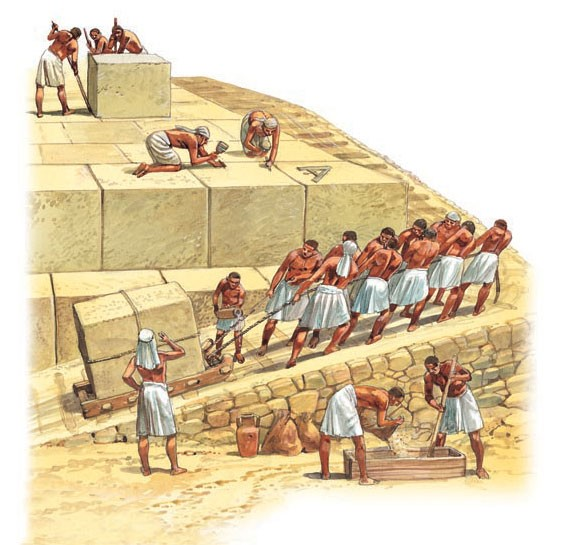
\includegraphics[width=\textwidth]{img/pyramids.jpg}
\end{column}
\end{columns}
\end{frame}


\section{Introduction to Flix}

\begin{frame}{The Flix Programming Language (1/2)}
A \textbf{functional}, \textbf{imperative}, and \textbf{declarative} logic
programming language.

\begin{itemize}
    \item Developed at Aarhus University in collaboration with programming
    language researchers from Waterloo (Canada), T\"ubingen (Germany), and
    Copenhagen.
    \item My personal research project. 
\end{itemize}

Free, open source, and ready for use:

\begin{center}
    \url{https://flix.dev/}
\end{center}
\end{frame}

\begin{frame}{The Flix Programming Language (2/2)}
Flix is an \textbf{advanced} programming language with a \textbf{unique}
combination of \textbf{powerful} programming language features: 

\small
\begin{columns}
\begin{column}{.55\textwidth}
\begin{itemize}
    \item algebraic data types and pattern matching 
    \item tuples and extensible records 
    \item parametric polymorphism
    \item type classes (traits)
    \item higher-kinded and associated types
    \item type match and purity reflection
    \item a polymorphic effect system 
\end{itemize}
\end{column}
\begin{column}{.45\textwidth}
\begin{itemize}
    \item scoped mutable state
    \item structured concurrency
    \item channels and processes
    \item first-class Datalog programs
    \item local type inference
    \item full tail call elimination
    \item and more ...
\end{itemize}
\end{column}
\end{columns}
\end{frame}

\section{First-Class Datalog Programs}

\begin{frame}[fragile]{Motivation (1/2)}
Given the Datalog facts:

\begin{lstlisting}[language=flix, xleftmargin=0.8cm]
ParentOf("Pompey", "Strabo").
ParentOf("Gnaeus", "Pompey").
ParentOf("Pompeia", "Pompey").
ParentOf("Sextus", "Pompey").
\end{lstlisting}

\pause

We can compute the ancestor of every person:

\begin{lstlisting}[language=flix, xleftmargin=0.8cm]
AncestorOf(x, y) :- ParentOf(x, y).
AncestorOf(x, z) :- AncestorOf(x, y), AncestorOf(y, z).
\end{lstlisting}
\end{frame}

\begin{frame}[fragile]{Motivation (2/2)}
Given the additional facts:

\begin{lstlisting}[language=flix, xleftmargin=0.8cm]
AdoptedBy("Augustus", "Caesar").
AdoptedBy("Tiberius", "Augustus").
\end{lstlisting}

We can extend the original program to include adoptions:

\begin{lstlisting}[language=flix, xleftmargin=0.8cm]
AncestorOf(x, y) :- AdoptedBy(x, y).
\end{lstlisting}

\pause

This example demonstrates the \emph{elegance} of Datalog:

\begin{itemize}
    \item We can extend the meaning of a program by adding new rules.
    \item i.e. we have extension by \emph{addition}, not by \emph{modification}.
\end{itemize}
\end{frame}

\begin{frame}{The Problem}
But now we have \textbf{\emph{two}} programs: 

\begin{itemize}
    \item one with biological parents, and
    \item one with biological parents and adoptions.
\end{itemize}

\pause

How do we \textbf{maintain} and \textbf{develop} these programs?

\begin{itemize}
    \pause \item With separate copies? $\Rightarrow$ \textcolor{red}{\bfseries multiple maintenance problem?}
    \pause \item With textual generation? $\Rightarrow$ \textcolor{red}{\bfseries correctness? expressive power?}
    \pause \item With procedural macros? $\Rightarrow$ \textcolor{red}{\bfseries correctness? expressive power?}
\end{itemize}

\pause

\begin{center}
\large
\textbf{Idea:} Datalog programs as a \emph{first-class} values.
\end{center}
\end{frame}

\begin{frame}[fragile]{Example (1/2)}
We define a function which returns a Datalog program value:

\begin{lstlisting}[language=flix, xleftmargin=0.8cm]
def getAncestors(withAdoptions: Bool): #{ ... } =
    let p1 = #{
        AncestorOf(x, y) :- ParentOf(x, y).
        AncestorOf(x, z) :- AncestorOf(x, y), AncestorOf(y, z).
    };
    let p2 = #{
        AncestorOf(x, y) :- AdoptedBy(x, y). 
    };
    if (withAdoptions) (p1 <+> p2) else p1
\end{lstlisting}

If \Code{withAdoptions} is \Code{true} we return the extended program with
adoptions. Otherwise we return the original program with only biological
parents. 
\end{frame}

\begin{frame}[fragile]{Example (2/2)}
We can use the \Code{getAncestors} as follows:

\begin{lstlisting}[language=flix, xleftmargin=0.8cm]
def main(): Unit \ IO = 
    let db = #{
      ParentOf("Pompey", "Strabo").
      ParentOf("Gnaeus", "Pompey").
      ParentOf("Pompeia", "Pompey").
      ParentOf("Sextus", "Pompey").
      AdoptedBy("Augustus", "Caesar").
      AdoptedBy("Tiberius", "Augustus").
    };
    let r = query db, getAncestors(true) 
            select x from AncestorOf("Tiberius", x);
    println(r)
\end{lstlisting}

which prints \Code|Vector#{Augustus, Caesar}|.
\end{frame}

\begin{frame}{First-Class Datalog Programs}
We propose the idea of \textbf{first-class Datalog programs}:

\begin{itemize}
    \item A \emph{Datalog program value} is a set of Datalog facts and rules.
    \item Datalog programs can be passed as arguments, stored in local
    variables, returned, and composed with other Datalog programs.
\end{itemize}

\pause

We can \textbf{construct}, \textbf{compose}, and \textbf{query} Datalog programs.

\begin{itemize}
    \item The solution to Datalog program value is its minimal model.
    \item The minimal model is itself a Datalog program value.
\end{itemize}

\textbf{Upshot:} We can create pipelines of Datalog programs.
\end{frame}

\begin{frame}[fragile]{Fundamental Operations}
\textbf{Datalog Literals}
\begin{itemize}
    \small
    \item A Datalog literal is written with bracket syntax \Code|#{...}|.
\end{itemize}

\pause

\textbf{Injection} --- Getting facts into Datalog
\begin{itemize}
    \small
    \item The \Code{inject e1, ..., en into A1, ... An} expression returns a
    Datalog program where each tuple in the collection $e_i$ is associated with
    predicate symbol $A_i$.
\end{itemize}

\pause

\textbf{Composition}
\begin{itemize}
    \small
    \item The \Code|e1 <+> e2| expression combines two Datalog programs $e_1$
    and $e_2$.
\end{itemize}

\pause

\textbf{Solving} --- Getting facts out of Datalog
\begin{itemize}
    \small
    \item The \Code{query e1, ..., en select (x1, ..., xm) from A1, ..., A_o}
    expression computes the minimal model of the expressions $e_1, \cdots, e_n$
    and then it selects the variables $x_1, \cdots, x_m$ from the relations
    $A_1, \cdots, A_o$. The result is a \Code{Vector} of tuples.
\end{itemize}
\end{frame}

\begin{frame}[fragile]{Datalog Literals (1/3)}
A Datalog literal is written\footnote{The empty Datalog literal 
%
\lstinline{\#\{ \}} 
%
is a legal Datalog program value.}:

\begin{lstlisting}[language=flix, xleftmargin=0.8cm]
#{ ... }
\end{lstlisting}

\pause

A Datalog literal may contain facts:

\begin{lstlisting}[language=flix, xleftmargin=0.8cm]
#{ A(1). A(2). A(3). B(42). }
\end{lstlisting}

\pause

A Datalog literal may contain rules:

\begin{lstlisting}[language=flix, xleftmargin=0.8cm]
#{ A(x) :- B(x), C(x). }
\end{lstlisting}
\end{frame}

\begin{frame}[fragile]{Datalog Literals (2/3)}
A Datalog literal may contain both facts and rules:

\begin{lstlisting}[language=flix, xleftmargin=0.8cm]
#{ A(1). 
   A(2). 
   B(1).
   C(x) :- A(x), B(x). }
\end{lstlisting}

A Datalog program is \emph{inert} until its minimal model is evaluated with
\Code{query}. 

\begin{itemize}
    \item i.e. in the above Datalog literal the fact \lstinline{C(1)} is
    \emph{not} automatically derived. 
\end{itemize}
\end{frame}

\begin{frame}[fragile]{Datalog Literals (3/3)}
Datalog program values are first-class:

\begin{itemize}
    \item We can store them in local variables.
    \item We can pass them as arguments to functions.
    \item We can return them from functions.
    \item We can store them inside data structures (e.g. in lists, maps).
\end{itemize}

\pause

Datalog program values do \emph{not} implement any traits.

\begin{itemize}
    \item In particular they do \emph{not} implement \Code{Eq[t]} nor \Code{Order[t]}.
    \item Hence, we can only manipulate them using \Code{query}.
\end{itemize}
\end{frame}

\begin{frame}[fragile]{Values as Terms}
Primitive values are permitted as terms:

\begin{lstlisting}[language=flix, xleftmargin=0.8cm]
#{ A(1, 2, 3). };           // OK
#{ A("Hello"). };           // OK
\end{lstlisting}

\pause

Compound values are also permitted as terms:

\begin{lstlisting}[language=flix, xleftmargin=0.8cm]
#{ A((1, 1), (2, 2)). };    // OK
#{ A(Set#{1, 2, 3}). };     // OK
\end{lstlisting}

Any type which implements \Code{Eq[t]} and \Code{Order[t]} can be used as a
term.

\pause

\textbf{Question:} What types are then excluded?
\end{frame}

\begin{frame}[fragile]{Lexical Scope (1/2)}
Datalog literals integrate with lexical scope.

For example, we can capture variables from lexical scope:

\begin{lstlisting}[language=flix, xleftmargin=0.8cm]
def mkParentOf(c: String, p: String): #{ ... } = 
  #{ ParentOf(c, p). }
\end{lstlisting}

Here $c$ and $p$ are Flix program variables, \emph{not} Datalog variables. 

\pause

We can use \Code{mkParentOf} to write:

\begin{lstlisting}[language=flix, xleftmargin=0.8cm]
mkParentOf("Pompey", "Strabo") <+> mkParentOf("Sextus", "Pompey")
\end{lstlisting}

to construct a Datalog program with two \Code{ParentOf} facts in it.
\end{frame}

\begin{frame}[fragile]{Lexical Scope (2/2)}
We can take this idea further and write a function to convert a list of pairs
into a Datalog program value with \Code{ParentOf} facts: 

\begin{lstlisting}[language=flix, xleftmargin=0.8cm]
def mkParentOf(l: List[(String, String)]): #{ ... } = 
    match l {
        case Nil          => #{}
        case (c, p) :: xs => 
            #{ ParentOf(c, p). } <+> mkParentOf(xs)
    }
\end{lstlisting}

\pause

This works, but ...

\textbf{Problem:} Writing such functions for every data type can get tedious.
\end{frame}

\begin{frame}[fragile]{Injecting Facts (1/4)}
We have an \textbf{impedance mismatch} between functional programming and Datalog:

\begin{itemize}
    \item Functional languages uses data structures: lists, sets, and maps.
    \item Datalog uses relations, i.e. sets of facts.
\end{itemize}

\pause

How can we reconcile the two? 

\begin{itemize}
    \item We need a mechanism to translate between data structures and
    relations. 
\end{itemize}

We introduce the \Code{inject} construct as mechanism to associate a collection
with a predicate symbol and to translate it into a Datalog representation.
\end{frame}

\begin{frame}[fragile]{Injecting Facts (2/4)}
For example, we can translate a list of tuples:

\begin{lstlisting}[language=flix, xleftmargin=0.8cm]
let edges = (1, 2) :: (2, 3) :: (3, 3) :: Nil
\end{lstlisting}

into a Datalog relation, i.e. a set of facts, using \Code{inject}:

\begin{lstlisting}[language=flix, xleftmargin=0.8cm]
inject edges into Edge
\end{lstlisting}

which evaluates to the Datalog program value:

\begin{lstlisting}[language=flix, xleftmargin=0.8cm]
#{ Edge(1, 2). Edge(2, 3). Edge(3, 3). }
\end{lstlisting}
\end{frame}

\begin{frame}[fragile]{Injecting Facts (3/4)}
We can use \Code{inject} to translate multiple heterogeneous collections into
relations.

For example, 

\begin{lstlisting}[language=flix, xleftmargin=0.8cm]
let nodes = Set#{1, 2, 3, 4};
let edges = (1, 2) :: (2, 3) :: (3, 3) :: Nil
inject nodes, edges into Node, Edge
\end{lstlisting}

evaluates to the Datalog program value:

\begin{lstlisting}[language=flix, xleftmargin=0.8cm]
#{ Node(1). Node(2). Node(3). Node(4). 
   Edge(1, 2). Edge(2, 3). Edge(3, 3). }
\end{lstlisting}
\end{frame}

\begin{frame}[fragile]{Injecting Facts (4/4)}
The general form of \Code{inject} is:

\begin{lstlisting}[language=flix, xleftmargin=0.8cm]
inject exp_1, exp_2, ... exp_n into sym_1, sym_2, ..., sym_n
\end{lstlisting}

The \Code{inject} construct works for any collection that implements
\Code{Foldable[t]}. 

\begin{itemize}
    \item E.g. \texttt{List[t]}, \texttt{Set[t]} and \texttt{Map[k, v]}, and many more...
\end{itemize}

\pause

\textbf{Upshot:} \Code{Foldable[t]} can be implemented for user-defined data
types, hence \Code{inject} builds upon an extensible foundation.
\end{frame}


\begin{frame}[fragile]{Composition}
We have already seen that we can compose Datalog programs with:

\begin{lstlisting}[language=flix, xleftmargin=0.8cm]
s1 <+> s2
\end{lstlisting}

which evaluates to the union of the constraints in both $s_1$ and $s_2$.

Composition is a well-behaved operation since the order of constraints in a
Datalog program value is immaterial. 

Composition is a low-level operation and we rarely use it directly.
\end{frame}

\begin{frame}[fragile]{Querying the Minimal Model (1/3)}
Given a Datalog program value:

\begin{lstlisting}[language=flix, xleftmargin=0.8cm]
let p = #{ A(1). A(2). B(x) :- A(x). }
\end{lstlisting}

We can compute its minimal model with \Code{query} and extract all its \Code{B}
facts:

\begin{lstlisting}[language=flix, xleftmargin=0.8cm]
query p select x from B(x) 
\end{lstlisting}

which evaluates to the the vector:

\begin{lstlisting}[language=flix, xleftmargin=0.8cm]
Vector#{ 1, 2 }
\end{lstlisting}
\end{frame}

\begin{frame}[fragile]{Querying the Minimal Model (2/3)}
Given two Datalog program values:
    
\begin{lstlisting}[language=flix, xleftmargin=0.8cm]
let db = #{ A(1). A(2).   }
let pr = #{ B(x) :- A(x). }
\end{lstlisting}

We can use query to compose them and compute their minimal model:

\begin{lstlisting}[language=flix, xleftmargin=0.8cm]
query db, pr select x from B(x) 
\end{lstlisting}

which, as before, evaluates to:

\begin{lstlisting}[language=flix, xleftmargin=0.8cm]
Vector#{ 1, 2 }
\end{lstlisting}
\end{frame}

\begin{frame}[fragile]{Querying the Minimal Model (3/3)}
We can use \Code{query} for more complex queries.

For example, given: 

\begin{lstlisting}[language=flix, xleftmargin=0.8cm]
let p = #{ A(1). A(2). A(3), B(1, 2). }
\end{lstlisting}

We can write the more interesting query:

\begin{lstlisting}[language=flix, xleftmargin=0.8cm]
query p select (x, y + 1) from A(x), A(y), B(x, y) where x > 0 
\end{lstlisting}

which evaluates to the vector:

\begin{lstlisting}[language=flix, xleftmargin=0.8cm]
Vector#{ (1, 3) }
\end{lstlisting}
\end{frame}

\begin{frame}[fragile]{Inject and Query}

We have seen how \Code{inject} and \Code{query} bridge the gap between Datalog
and Flix:

\begin{itemize}
    \item We can use \Code{inject} to translate any data type, which implements
    the \Code{Foldable} trait, into a set of Datalog facts, and 
    \item We can use \Code{query} to compute the minimal model of a collection
    of Datalog program values, and to extract tuples as an immutable
    \Code{Vector}.
\end{itemize}

\textbf{Upshot:} We can easily transport data into and out of the Datalog world.
\end{frame}

\begin{frame}[fragile]{Example I}
What does the following program print?

\begin{lstlisting}[language=flix, xleftmargin=0.8cm]
def main(): Unit \ IO = 
    let p1 = #{ Edge(1, 2). Edge(2, 3). };
    let p2 = #{ 
        Edge(y, x) :- Edge(x, y). 
    };
    let p3 = #{ 
        Path(x, y) :- Edge(x, y).
        Path(x, z) :- Path(x, y), Edge(y, z).
    };
    let result = query p1, p2, p3 select (a, b) from Edge(a, b);
    println(result)
\end{lstlisting}
\end{frame}

\begin{frame}[fragile]{Example II: Trick Question}
What does the following program print?

\begin{lstlisting}[language=flix, xleftmargin=0.8cm]
def main(): Unit \ IO = 
    let x = #{ Leg("BLL", "LH", "FRA"). Leg("FRA", "LH", "YYZ"). 
               Leg("YYZ", "AC", "YVR"). Leg("YYZ", "AC", "SFO"). };
    let y = #{ 
        Route(x, a, y) :- Leg(x, a, y).
    };
    let z = #{ 
        Route(x, a, z) :- Route(x, a, y), Leg(y, a, z).
    };
    let result = query x, z select (src, dst) from Leg(src, dst);
    println(result)
\end{lstlisting}

% We have 4 issues: 2 are type system related and 2 are logical:
% - Types: We have x bound by lexical scope in the def. of y and z.
% - Types: The Leg predicate has arity 3, not 2.
% - Logic: We were supposed to query Route, not Leg.
% - Logic: We forgot to query the program y.
\end{frame}

\section{A Type System for First-class Datalog}

\begin{frame}{Why a Type System?}
The Flix type system gives us three important properties:

\begin{itemize}
    \item (\textbf{Safety}) Well-typed programs cannot go wrong.
    \item (\textbf{Synthesis}) Automatic resolution and derivation of code via
    traits. 
    \item (\textbf{IDE Support}) Auto-complete, automatic refactoring, etc.
\end{itemize}

\medskip

\small
\textbf{Footnote:} Flix also has an \emph{effect system} which enables enforcement of purity.
\end{frame}

\begin{frame}{What could possibly go wrong? (1/3)}
\begin{center}
    % https://www.dailymail.co.uk/news/article-3091148/Chilling-image-shows-miners-playing-asbestos-shovelling-competition.html
    %
    % Shockingly, all of the men in the image but one have died from asbestos
    % related diseases, with several also losing their children from exposure to
    % the deadly mineral.
    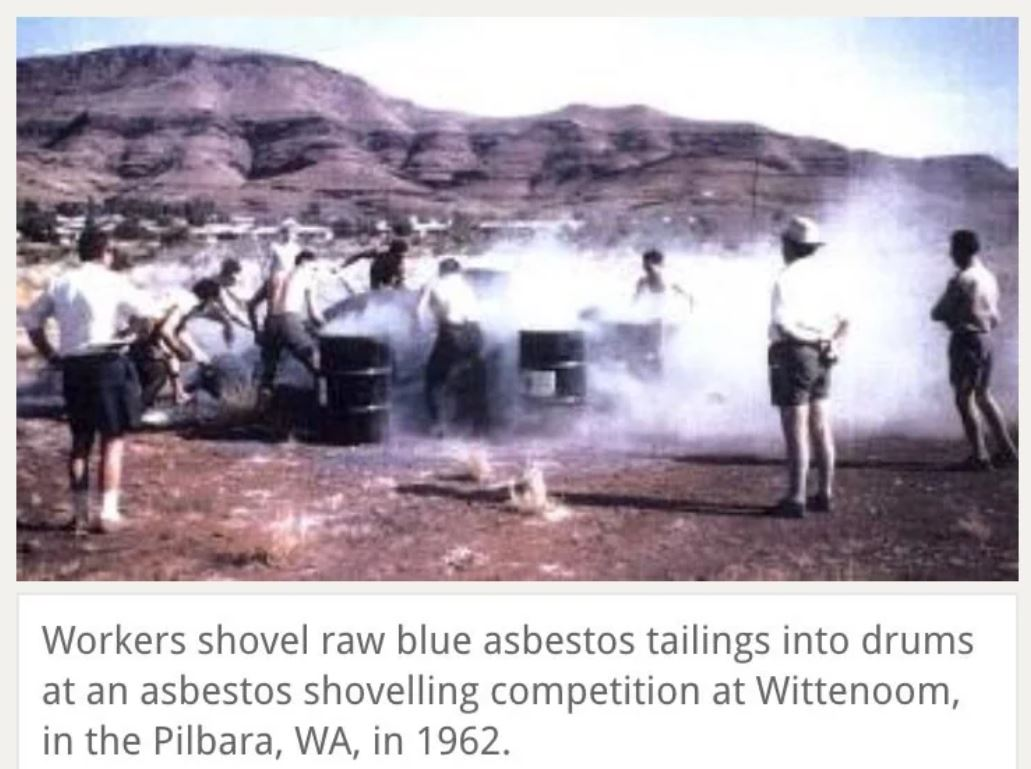
\includegraphics[width=0.7\textwidth]{img/asbestos.jpg}
\end{center}
\end{frame}  

\begin{frame}[fragile]{What could possibly go wrong? (2/3)}
We want to ensure that programmers do not confuse \textbf{term types}:

\begin{lstlisting}[language=flix, xleftmargin=0.8cm]
let p1 = #{ Edge(1, 2). };
let p2 = #{ Edge("Aarhus", "Copenhagen"). };
p1 <+> p2
\end{lstlisting}

\pause

If we try to compile this program, Flix reports:

\begin{lstlisting}[language=flix, xleftmargin=0.8cm]
>> Unable to unify the types: 'Int32' and 'String'.

3 |     p1 <+> p2
        ^^^^^^^^^
        mismatched types.
\end{lstlisting}
\end{frame}

\begin{frame}[fragile]{What could possibly go wrong? (3/3)}
We also want to ensure that programmers do not confuse \textbf{predicate arity}:

\begin{lstlisting}[language=flix, xleftmargin=0.8cm]
let p1 = #{ Edge(1, 2). };
let p2 = #{ Edge(1, 2, 3). };
p1 <+> p2
\end{lstlisting}

\pause

If we try to compile this program, Flix reports:

\begin{lstlisting}[language=flix, xleftmargin=0.8cm]
>> Unable to unify the types: '(?, ?)' and '(Int32, ?, ?)'.

3 |     p1 <+> p2
        ^^^^^^^^^
        mismatched types.

\end{lstlisting}
\end{frame}

\begin{frame}{Polymorphic Type Systems}
You are probably already familiar with two types of polymorphism:

\begin{itemize}
    \item \textbf{Subtype polymorphism} --- ``inheritance''
    \item \textbf{Parametric polymorphism} --- ``generics''
\end{itemize}

\pause

Flix uses another kind of polymorphism to type Datalog programs:

\begin{itemize}
    \item \textbf{Row polymorphism}
\end{itemize}
\end{frame}

\begin{frame}[fragile]{Row Types}
A row type is of the form:
$$
\rho = \alpha \mid \epsilon \mid \left \{ p (\tau_1, \cdots, \tau_n) \mid \rho \right \}
$$
where $\tau$ is a collection of base types (e.g. \Code{Bool}, \Code{Int32}, \Code{String}).

\medskip

\pause

We consider rows equivalent up to associativity and commutativity. 

\medskip

\scriptsize
\textbf{Note:} The Flix type system ensures that a predicate symbol $p$ can
occur at most once in a row.
\end{frame}

\begin{frame}[fragile]{Example (1/3)}
The Datalog program:
%
\begin{lstlisting}[language=flix, xleftmargin=0.8cm]
#{ A(1, 2). B("Hello"). }
\end{lstlisting}    
%
has the type:
%
\[
\forall \alpha. \left\{ A(\textsf{Int32}, \textsf{Int32}) \mid \left\{ B(\textsf{String}) \mid \alpha \right\} \right\}
\]
%
\pause but it also has the \emph{equivalent} type:
%
\[
\forall \alpha. \left\{ B(\textsf{String}) \mid \left\{ A(\textsf{Int32}, \textsf{Int32}) \mid \alpha \right\} \right\}
\]
%
\pause and more interestingly it also has the \emph{less general} type:
%
\[
\forall \alpha. \left\{ A(\textsf{Int32}, \textsf{Int32}) \mid \left\{ B(\textsf{String}) \mid \left\{ C(\textsf{Bool}) \mid \alpha \right\} \right\} \right\}
\]
%
\end{frame}

\begin{frame}[fragile]{Example (2/3)}
The Datalog program:
%
\begin{lstlisting}[language=flix, xleftmargin=0.8cm]
#{ Path(x, y) :- Edge(x, y). }
\end{lstlisting}    
%
has the type:
%
\[
\forall a, b, \alpha. \left\{ \textsf{Edge}(a, b) \mid \left\{ \textsf{Path}(a, b) \mid \alpha \right\} \right\}
\]
%
\pause whereas the Datalog program:
%
\begin{lstlisting}[language=flix, xleftmargin=0.8cm]
#{ Path(x, z) :- Path(x, y), Edge(y, z) }
\end{lstlisting}    
%
\pause has the type:
%
\[
\forall a, b, \alpha. \left\{ \textsf{Edge}(\underline{b}, b) \mid \left\{ \textsf{Path}(a, b) \mid \alpha \right\} \right\}
\]
%
\end{frame}

\begin{frame}[fragile]{Example (3/3)}
The two Datalog programs
%
\begin{lstlisting}[language=flix, xleftmargin=0.8cm]
let p1 = #{ A(1). A(2). A(3). };
let p2 = #{ B(1). B(2). B(3). };
\end{lstlisting}    
%
have the types:
%
\[
\forall \alpha_1. \left\{ A(\textsf{Int32}) \mid \alpha_1 \right\}
\qquad \text{and} \qquad
\forall \alpha_2. \left\{ B(\textsf{Int32}) \mid \alpha_2 \right\}
\]
%
\pause Hence the composition \Code{p1 <+> p2} has the type:
%
\[
\forall \alpha_3. \left\{ A(\textsf{Int32}) \mid \left\{ B(\textsf{Int32}) \mid \alpha_3 \right\} \right\}
\]
%
\end{frame}

\begin{frame}[fragile]{Pitfall (1/2)}
The following does not work: 

\begin{lstlisting}[language=flix, xleftmargin=0.8cm]
def f(): #{ Edge(Int32, Int32) } = #{ Edge(1, 2). }
def g(): #{ Path(Int32, Int32) } = #{ Path(2, 3). }
def h(): #{ Edge(Int32, Int32), Path(Int32, Int32) } = 
    f() <+> g()
\end{lstlisting}

\pause Specifically, the Flix compiler reports:

\begin{lstlisting}[language=flix, xleftmargin=0.8cm]
>> Missing predicate 'Edge' of type 'Relation(Int32, Int32)'.

4 |     f() <+> g()
        ^^^^^^^^^^^
        missing predicate.
\end{lstlisting}
\end{frame}

\begin{frame}[fragile]{Pitfall (2/2)}
We we should have done is to use \textbf{open rows}:

\begin{lstlisting}[language=flix, xleftmargin=0.8cm]
def f(): #{ Edge(Int32, Int32) | r } = #{ Edge(1, 2). }
def g(): #{ Path(Int32, Int32) | r } = #{ Path(2, 3). }
def h(): #{ Edge(Int32, Int32), Path(Int32, Int32) | r} = 
    f() <+> g()
\end{lstlisting}

Here, because each row is open, we can build bigger rows.
\end{frame}

\begin{frame}{Summary}
\textbf{Beyond Datalog}: Datalog programs as first-class values in Flix:

\begin{itemize}
    \item Datalog programs are \emph{values}. We can pass them around.
    \item Datalog literals may capture variables from the lexical scope.
    \item Use \Code{inject} to translate data structures to Datalog facts.
    \item Use \Code{query} to compute minimal models and to extract facts.
    \item A row polymorphic type system ensures safety.
\end{itemize}

\textbf{Upshot:} We can create modular and reusable families of Datalog programs.
\end{frame}

\begin{frame}[standout]
% blank
\end{frame}

\begin{frame}{Week 2: Outline}
\color{gray}
\begin{columns}
\begin{column}{.05\textwidth}
\rotatebox{90}{\large \textbf{\DayOne{}}}
\end{column}
\begin{column}{.95\textwidth}
    \footnotesize
\textbf{Lecture} (45min)  \vspace{-2mm}
\begin{itemize}
    \color{gray}
    \setlength\itemsep{-0.5em}
    \item Datalog programs as first-class values in a general-purpose language.
    \item A row polymorphic type system for Datalog program values.
\end{itemize}
\textbf{Exercises} (45min) \vspace{-2mm}
\begin{itemize}
    \color{gray}
    \item Work on the assignment alone or together in small groups.
\end{itemize}
\end{column}
\end{columns}

\medskip
\medskip
\medskip

\color{black}
\begin{columns}
\begin{column}{.05\textwidth}
\rotatebox{90}{\large \textbf{\DayTwo{}}}
\end{column}
\begin{column}{.95\textwidth}
\footnotesize
\textbf{Lecture} (45min) \vspace{-2mm}
\begin{itemize}
    \setlength\itemsep{-0.5em}
    \item Datalog program values and rho abstraction.
    \item Datalog extended with lattice semantics.
    \item Computing provenance information.
\end{itemize}
\textbf{Exercises} (45min)  \vspace{-2mm}
\begin{itemize}
    \item Work on the assignment alone or together in small groups.
\end{itemize}
\end{column}
\end{columns}
\end{frame}

\begin{frame}{Quote of the Day}
``Every program is a part of some other program and rarely fits.''

\begin{flushright}
--- Alan Perlis
\end{flushright}
\end{frame}

\begin{frame}{Pull Requests are Welcome}
\begin{columns}
\begin{column}{.50\textwidth}
You can improve the course material!

\begin{itemize}
    \item Exercises are in \texttt{src/weekX.md}
    \item Slides are in \texttt{slides/weekX.tex}
\end{itemize}

\medskip

PRs can be submitted on GitHub:
\begin{center}
\scriptsize
\url{https://github.com/magnus-madsen/advprog/}
\end{center}
\end{column}
\begin{column}{.50\textwidth}
    % Source: https://www.q-files.com/history/ancient-egypt/pyramids-how-they-were-built
    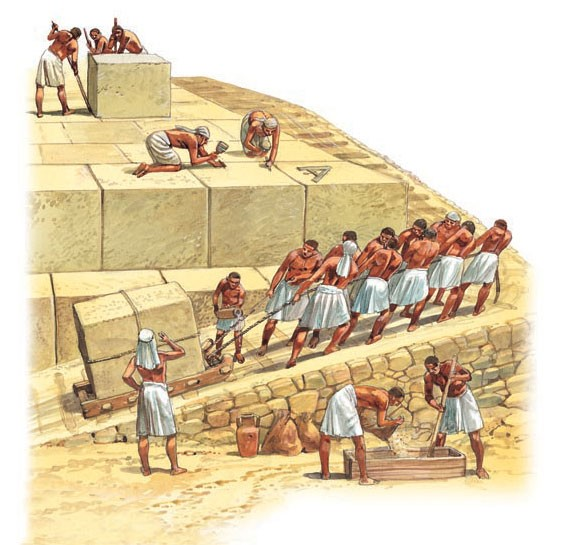
\includegraphics[width=\textwidth]{img/pyramids.jpg}
\end{column}
\end{columns}
\end{frame}


\section{Rho Abstraction}

\begin{frame}[fragile]{Motivation (1/2)}
We have seen how Datalog programs can be typed with row types:
%
\begin{lstlisting}[language=flix, xleftmargin=0.8cm]
def reach(): #{ Edge(t, t), Path(t, t) | r} = #{
    Path(x, y) :- Edge(x, y).
    Path(x, z) :- Path(x, y), Edge(y, z).
}
\end{lstlisting}
\end{frame}

\begin{frame}[fragile]{Motivation (2/2)}
But such types can quickly become unwieldy:
%
\begin{lstlisting}[language=flix, xleftmargin=0.8cm]
def disconnected(): 
    #{ Edge(t, t), Path(t, t), Vertex(t), Disconnected(t, t) | r} = #{
        Vertex(x)  :- Edge(x, _).
        Vertex(y)  :- Edge(_, y).
        Path(x, y) :- Edge(x, y).
        Path(x, z) :- Path(x, y), Edge(y, z).
        Disconnected(x, y) :- Vertex(x), Vertex(y), not Path(x, y).
    }
\end{lstlisting}

\pause

\textbf{Observation:} The \Code{Vertex} and \Code{Path} relations are really
internally implementations.

\pause

\textbf{Idea:} What do we usually do with internal implementation details? \textbf{\emph{We hide them.}}
\end{frame}

\begin{frame}[fragile]{Rho Abstraction}
We introduce \emph{rho abstraction} as a mechanism to \emph{hide} predicate symbols.

\small
\begin{itemize}
    \item A rho abstraction is of the form \Code{#(A, ...) -> e} where $e$ must
    be a Datalog expression.
    \pause \item A rho abstraction hides, by renaming, all predicate symbols \emph{not}
    listed in the argument list. 
    \pause \item The row type of a rho abstraction includes only those predicates in
    the argument list. 
    \pause \item Evaluation of a rho abstraction renames all hidden predicate symbols
    with fresh names. 
\end{itemize}

\pause

\textbf{Example:} \Code|#(A, B) -> #{A(123). C("a").}| evaluates to \Code|#{A(123). C17("a").}|. 
where \Code{C17} is a fresh predicate symbol that has never been used before.
\end{frame}

\begin{frame}[fragile]{Rho Abstraction: The Wrong Way}
We may think that we can statically rename abstracted predicate symbols:

\begin{lstlisting}[language=flix, xleftmargin=0.8cm]
def disconnected(): #{ Edge(t, t), Disconnected(t, t) | r} = 
    #(Edge, Disconnected) -> #{
        Vertex17(x) :- Edge(x, _).
        Vertex17(y) :- Edge(_, y).
        // ... omitted for brevity ...
    }
\end{lstlisting}

\pause

\textbf{But this does not work.} Why?

\pause

\begin{lstlisting}[language=flix, xleftmargin=0.8cm]
let p1 = #(A) -> (#{ Edge(123, 456). } <+> disconnected());
let p2 = #(A) -> (#{ Edge("a", "b"). } <+> disconnected());
query p1, p2 ...
\end{lstlisting}

\textbf{Oops.} Now the Datalog program contains the facts \Code{Vertex17(123)}
and \Code{Vertex17("a")} -- which is a type error! We must rename predicates at
\emph{runtime} to ensure fresh names!
\end{frame}

\begin{frame}[fragile]{Rho Abstraction: The Right Way}
Each evaluation of a rho abstraction introduces fresh names.

Hence, in the previous example, we get:

\begin{lstlisting}[language=flix, xleftmargin=0.8cm]
let p1 = #{ Vertex17(123). Vertex17(456). ... };
let p2 = #{ Vertex18("a"). Vertex18("b"). ... };
query p1, p2 ...
\end{lstlisting}

where there is no longer any type error between \Code{Vertex17(123)} and \Code{Vertex18("a")}.

\pause

\textbf{Upshot:} The abstracted predicate symbols have become truely local.
\end{frame}

\section{Datalog and Lattice Semantics}

\begin{frame}[fragile]{Motivation (1/4)}
We know how to compute reachability in a graph:

\begin{lstlisting}[language=flix, xleftmargin=0.8cm]
def reach(origin: t, edges: List[(t, t)]): Vector[t] with Order[t] = 
    let db = inject edges into Edge;
    let pr = #{
        Reach(origin).
        Reach(y) :- Reach(x), Edge(x, y).
    };
    query db, pr select x from Reach(x)
\end{lstlisting}

\pause

But, what if we wanted to compute the \textbf{shortest distance} to every vertex
from an origin, i.e. \emph{single-source shortest distance} (SSSD)?
\end{frame}

\begin{frame}[fragile]{Motivation (2/4)}
We can use \emph{lattice semantics} to solve this problem:

\begin{lstlisting}[language=flix, xleftmargin=0.8cm]
def sssd(origin: t, edges: List[(t, Int32, t)]): ... = 
    let db = inject edges into Edge;
    let pr = #{
        Dist(origin; Down(0)).
        Dist(y; d1 + Down(d2)) :- Dist(x; d1), Edge(x, d2, y).
    };
    query db, pr select (x, d) from Dist(x; d) |> Vector.toMap

def main(): Unit \ IO = 
    println(sssd("a", List#{("a", 2, "b"), ("b", 5, "c")}))
\end{lstlisting}

Prints \Code|Map#{a => 0, b => 2, c => 7}|.
\end{frame}

\begin{frame}[fragile]{Motivation (3/4)}
A lot is going on, so let us break it down.

\medskip

The fact: \Code{Dist(origin; Down(0)).}

\begin{itemize}
    \pause \item Asserts that \Code{Dist} is a (map) lattice, and \emph{not} a relation (the semicolon).
    \pause \item Asserts that the distance to the origin is at most zero. 
    \pause \item The \Code{Down} data type, which wraps zero, \emph{reverses} the order
    on \Code{Int32}.
\end{itemize}
\end{frame}

\begin{frame}[fragile]{Motivation (4/4)}
The rule: \Code|Dist(y; d1 + Down(d2)) :- Dist(x; d1), Edge(x, d2, y).|
%
\begin{itemize}
    \pause \item Asserts that \Code{Dist} is a (map) lattice, and \emph{not} a relation (as before).
    \pause \item Asserts that the distance to \Code{y} is \emph{at
    most}\footnote{Technically, it asserts that the distance is \emph{at least},
    but since the lattice order is reversed, \emph{at least} becomes \emph{at
    most}.} \Code{d1 + Down(d2)} \emph{if} the distance to \Code{x} is \Code{d1}
    and the distance on the edge from \Code{x} to \Code{y} is \Code{d2}.
\end{itemize}

\pause 

What if there are two paths leading to \Code{y} but with different distances?
In that case, we compute their \emph{join} which, according the reversed lattice
order, is the minimum of the two distances-- exactly what we want.
\end{frame}

\begin{frame}{From Relations to Lattices}

We have seen that Flix supports \emph{constraints on relations}. 

\begin{itemize}
    \item But now also \emph{constraints on lattices}.
\end{itemize}

We use the semicolon \Code{;} to indicate when we want lattice semantics.

\pause

A lattice has the following components:

\begin{itemize}
    \item Least and Greatest Elements (\Code{LowerBound} and \Code{UpperBound}).
    \item A partial order (\Code{Partial Order}).
    \item A least upper bound for any two elements (\Code{JoinLattice}).
    \item A greatest lower bound for any two elements (\Code{MeetLattice}).
\end{itemize}

which we define by implementing instances for the traits in parenthesis.

\end{frame}

\begin{frame}[fragile]{Joins and Meets}
\begin{columns}
\begin{column}{.5\textwidth}
Given the two facts:

\begin{lstlisting}[language=flix, xleftmargin=0.8cm]
A(1; Neg).
B(1; Pos).
\end{lstlisting}

The program:

\begin{lstlisting}[language=flix, xleftmargin=0.8cm]
P(x; l) :- A(x, l).
P(x; l) :- B(x, l).
Q(x; l) :- A(x; l), B(x; l).
\end{lstlisting}

\pause

Evaluates to a minimal model with:

\begin{lstlisting}[language=flix, xleftmargin=0.8cm]
P(1; Top).
\end{lstlisting}

\end{column}
\begin{column}{.5\textwidth}
\centering
\tikzset{node/.style={circle, fill=black!20, minimum size=4em, align=center}}
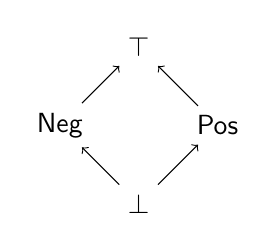
\begin{tikzpicture}
\node (T) at ( 0, 1) {$\top$};
\node (N) at (-1, 0) {\textsf{Neg}};
\node (P) at ( 1, 0) {\textsf{Pos}};
\node (B) at ( 0,-1) {$\bot$};

\path[->](N) edge node[left] {} (T);
\path[->](P) edge node[left] {} (T);
\path[->](B) edge node[left] {} (N);
\path[->](B) edge node[left] {} (P);
\end{tikzpicture}
\end{column}
\end{columns}

\medskip

\pause

{
\small
\textbf{Warning:} Do not mistake \Code{,} for \Code{;}. We must use \Code{;}
when we want lattice semantics. 
}

\end{frame}

\begin{frame}[fragile]{The \texttt{Down} Lattice (1/2)}
The \Code{Down} data type is defined as: 

\begin{lstlisting}[language=flix, xleftmargin=0.8cm]
pub enum Down[a] {
    case Down(a)
}
\end{lstlisting}

It defines instances for the traits \Code{PartialOrder}, \Code{LowerBound},
\Code{UpperBound}, \Code{JoinLattice}, and \Code{MeetLattice} under the
\emph{reverse} order on the underlying type \Code{a}.
\end{frame}

\begin{frame}[fragile]{The \texttt{Down} Lattice (2/2)}
For example, here are two instances:

\begin{lstlisting}[language=flix, xleftmargin=0.5cm]
instance PartialOrder[Down[a]] with PartialOrder[a] {
    pub def lessEqual(x: Down[a], y: Down[a]): Bool = 
        match (x, y) {
            case (Down.Down(xx), Down.Down(yy)) => 
                yy `PartialOrder.lessEqual` xx
    }
}

instance JoinLattice[Down[a]] with MeetLattice[a] {
    pub def leastUpperBound(x: Down[a], y: Down[a]): Down[a] = 
        match (x, y) {
            case (Down.Down(xx), Down.Down(yy)) => 
                Down.Down(xx `MeetLattice.greatestLowerBound` yy)
    }
}
\end{lstlisting}
\end{frame}

\begin{frame}[fragile]{Relation and Lattice Semantics}
We can combine relational and lattice semantics with a new form of
stratification: 

\begin{lstlisting}[language=flix, xleftmargin=0.8cm]
Degree("Kevin Bacon"; Down(0)).
Degree(x; n + Down(1)) :- Degree(y; n), StarsWith(y, x).
Layer(n; Set#{ x })    :- fix Degree(x; n).
Count(n, Set.size(s))  :- fix Layer(n; s)
\end{lstlisting}

\pause

This Datalog program computes how many actors are separated from Kevin Bacon by
$1, 2, 3, \cdots$ degrees. 

\pause

Importantly, the use of \Code{fix} enforces that \Code{Degree} is computed
before \Code{Layer} which is computed before \Code{Count}.
\end{frame}

\section{Computing Provenance}

\begin{frame}[fragile]{Motivation}
We have seen that we can compute shortest distances with lattice semantics: 

\begin{lstlisting}[language=flix, xleftmargin=0.8cm]
def sssd(origin: t, edges: List[(t, Int32, t)]): Map[t, Down[Int32]]
\end{lstlisting}

but what if we wanted to compute the \emph{shortest path} itself?
\end{frame}

\begin{frame}[fragile]{Shortest Paths: Attempt I}
What if we try:

\begin{lstlisting}[language=flix, xleftmargin=0.8cm]
Reach(origin, Nil; Down(0)).
Reach(y, y :: p; d1 + Down(d2)) :- Reach(x, p; d1), Edge(x, d2, y).
\end{lstlisting}

\textbf{Question:} What does this compute?

\pause

\textbf{Oops:} What if there are cycles?
\end{frame}
    
\begin{frame}[fragile]{Shortest Paths: Attempt II}
We need a new idea (ignoring distances for the moment).

We define a lattice on \emph{paths}:

\begin{itemize}
    \item The bottom element is the set of all infinite paths.
    \pause \item The top element is the empty path.
    \pause \item A path is smaller than another path if it is \emph{longer}, i.e. as we
    move \emph{up} the lattice, paths get shorter. 
\end{itemize}

\pause

\begin{lstlisting}[language=flix, xleftmargin=0.8cm]
Reach(origin; P(Nil)).
Reach(y; cons(y, p)) :- Reach(x; p), Edge(x, y).
\end{lstlisting}

where

\begin{lstlisting}[language=flix, xleftmargin=0.8cm]
enum P { case P(List[Int32]) }
\end{lstlisting}
\end{frame}

\begin{frame}[fragile]{Shortest Paths: Attempt II}
We define the \Code{PartialOrder} and \Code{JoinLattice} instances as:

\begin{lstlisting}[language=flix, xleftmargin=0.8cm]
instance PartialOrder[P] {
    pub def lessEqual(x: P, y: P): Bool = 
        let (P(xs), P(ys)) = (x, y);
        List.length(xs) >= List.length(ys)
}
instance JoinLattice[P] {
    pub def leastUpperBound(x: P, y: P): P = 
        let (P(xs), P(ys)) = (x, y);
        if (List.length(xs) <= List.length(ys)) x else y
}
\end{lstlisting}

\pause

\textbf{Question:} Do you see any problems here?

\pause

\textbf{Answer:} Comparing the two paths or computing their join is stupidly expensive!
\end{frame}

\begin{frame}[fragile]{Shortest Paths: Attempt III}
\textbf{Idea:}

\begin{itemize}
    \item We modify the lattice to track the path length \emph{implicitly}.
    \item We introduce an explicit bottom element: 
\end{itemize}

\begin{lstlisting}[language=flix, xleftmargin=0.8cm]
enum P {
    case P(Int32, List[Int32])
    case Bottom
}
\end{lstlisting}

\pause 

\textbf{Exercise:} Add instances for \Code{PartialOrder}, \Code{JoinLattice}, etc. for \Code{P}.
\end{frame}

\begin{frame}[fragile]{Example: Strongly Connected Components (1/2)}
\textbf{Problem:} We are given an undirected graph and we want to compute the SCCs.
\medskip
\begin{lstlisting}[language=flix, xleftmargin=0.8cm]
// `Reachable` is simply bi-directional reachability.
Reachable(n, n)   :- Node(n).
Reachable(n1, n2) :- Edge(n1, n2).
Reachable(n1, n2) :- Edge(n2, n1).
Reachable(n1, n2) :- Reachable(n1, m), Reachable(m, n2).
\end{lstlisting}
\end{frame}

\begin{frame}[fragile]{Example: Strongly Connected Components (2/2)}
\begin{lstlisting}[language=flix, xleftmargin=0.8cm]
// `ReachUp` contains nodes that can reach at least one other node 
// with a higher value. This contains all nodes that are not the 
// maximum node of their component.
ReachUp(n1) :- Reachable(n1, n2), if n1 < n2.

// `n` is in a component that is represented by `rep`.
// `rep` is the highest node of the component.
ComponentRep(n, rep) :- Reachable(n, rep), not ReachUp(rep).

// `Component(rep; c)` describes that the node `rep` is the 
// representative of the component `c` which is a set of nodes. 
Component(rep; Set#{n}) :- ComponentRep(n, rep).
\end{lstlisting}
\end{frame}

\begin{frame}{Summary}
We have seen several extensions that enrich Datalog in Flix:

\begin{itemize}
    \item Rho abstraction as a mechanism to hide predicate symbols.
    \item From \emph{constraints on relations}, to \emph{constraints on
    lattices}.
    \item How to compute provenance information with lattice semantics.
\end{itemize}
\end{frame}

\begin{frame}[standout]
% blank
\end{frame}

\end{document}
